%!TEX root = /Users/jakubkonka/Thesis/Thesis.tex
\chapter{Intelligent Network Selection} % (fold)
\label{cha:intelligent}

\minitoc
\vspace{10mm}

\section{The Problem of Intelligent Network Seletion} % (fold)
\label{sec:the_problem_of_intelligent_network_seletion_intelligent}
The aim of this section is to 

\subsection{Heterogeneous Wireless Access Network} % (fold)
\label{sub:heterogeneous_wireless_access_network_intelligent}
Over the last decade, the world of wireless and mobile communications has witnessed several major improvements \cite{ABC03}. The evolution of traditional 2$^\text{nd}$ Generation (2G) cellular systems (such as GSM), through 3$^{\text{rd}}$ Generation (3G) systems (such as UMTS or CDMA2000), into 4$^{\text{th}}$ Generation (4G) systems (such as LTE), has drastically improved the cellular coverage worldwide, and provided mobile Internet access \cite{HossainBeaubrun09, HossainTalebiFard09}. At the same time, IEEE 802.11-based Wireless Local Area Network (WLAN; commonly referred to as WiFi) solutions have emerged as the predominant high-speed wireless Internet access at airports, in hotels, or even at home.

With the introduction of smartphones (iPhones, Android phones, BlackBerry phones) and tablets (iPads, Android tablets), the wireless users are finally able to take advantage of both the coverage offered by 3G/4G cellular access network and the high-speed Internet access offered by WiFis. Whenever the smartphone/tablet is in close proximity to a WiFi hot spot, it automatically switches from 3G/4G to WiFi mode for faster data access. However, this only works when either the WiFi hot spot provides free access, or is within the user's subscription; for example, as part of the monthly data allowance plan with a local wireless access network operator. Moreover, this solution lacks the support for session continuity, and does not provide any intelligence when switching from one access network to another. For instance, although the WiFi hot spot is by definition deemed to offer faster data rates, this does not necessarily translate into higher Quality of Service (QoS). In fact, it might be just the contrary, especially in a very crowded hot spot area where the users run very bandwidth intensive applications such as video or music streaming, or even on-line gaming. For example, under such circumstances, trying to make a Skype call can be nearly impossible \cite{Wisely4gWLAN09}. Therefore, the decision to switch from one network to another should not only consider the availability of a particular wireless access network, but also the offered QoS for the best user experience.

\begin{figure}[t]
    \centering
    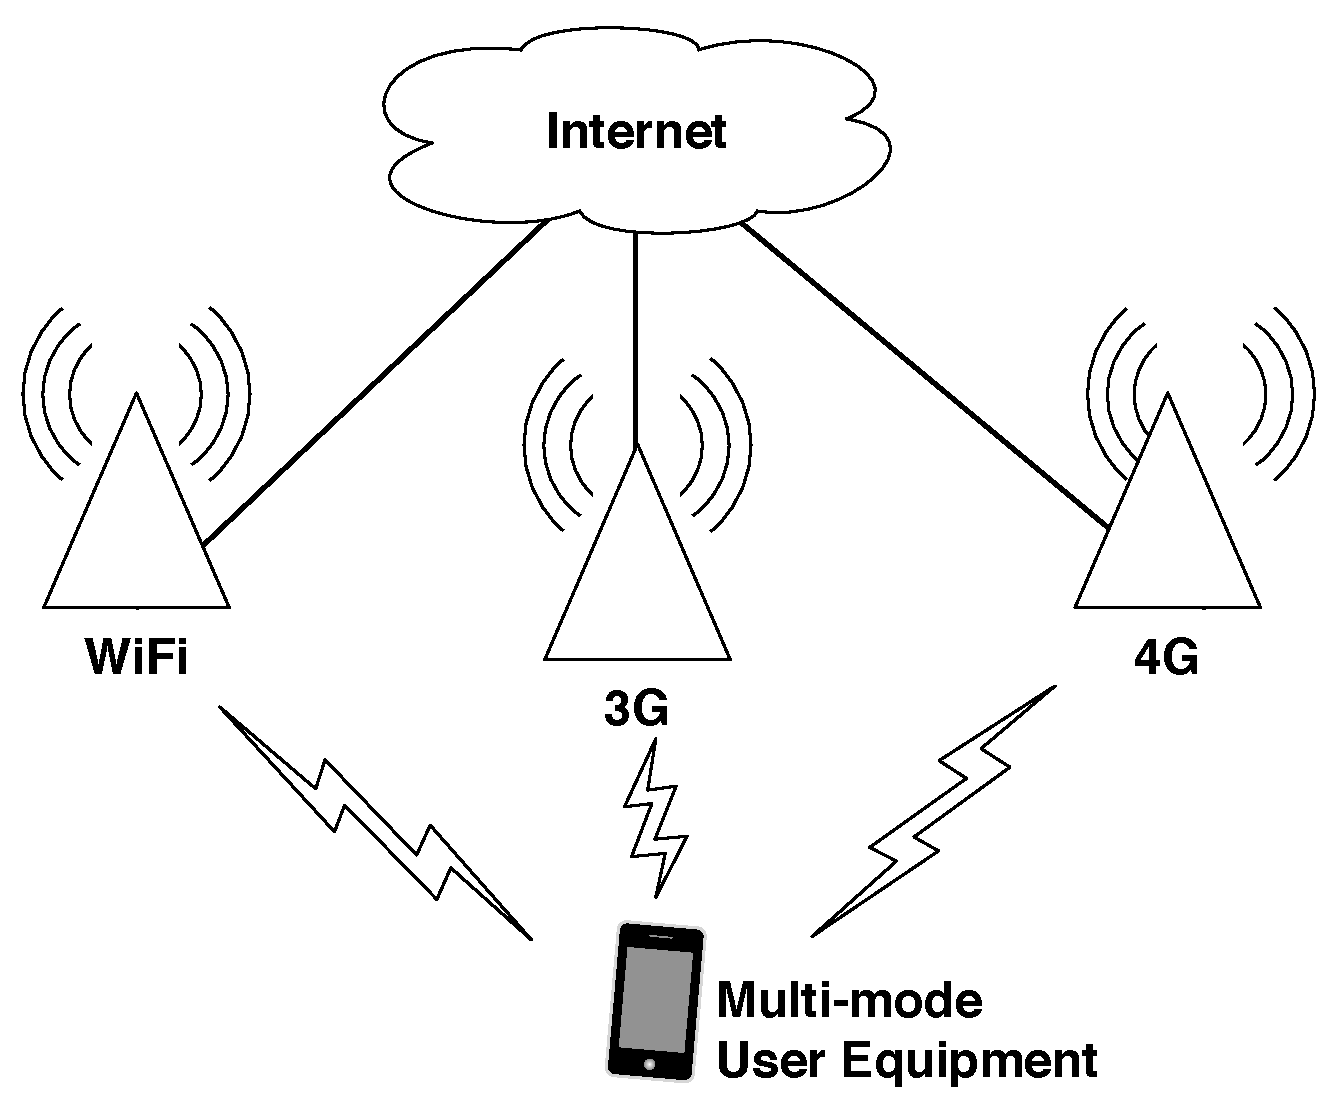
\includegraphics[width=3.5in]{Intelligent/Figures/heterogeneous}
    \caption{Heterogeneous wireless access network}
    \label{fig:heterogeneous_intelligent}
\end{figure}

This, together with the industry's drive to have an all-IP-based traffic, gives rise to the concept of a \emph{heterogeneous wireless access network}. The heterogeneous wireless access network spans different wireless access technologies integrated into one network to provide wireless and mobile users with the requested multimedia services and QoS. It will take full advantage of the multi-modality offered by the smartphones by having the device connected to all wireless access technologies at all times. This is depicted in Figure~\ref{fig:heterogeneous_intelligent}.

The heterogeneous wireless access network will possess many advantages over the contemporary wireless networking solution. From the users' perspective, different coverage and QoS characteristics of each of the included wireless access technologies will lead to the ability to seamlessly connect at any time, at any place, and to the access technology which offers the most optimal quality available. This is referred to as \emph{Always Best Connected} networking paradigm \cite{ABC03}, and will be introduced in more detail in the subsequent section. From the network operators' perspective, on the other hand, the integration of wireless access technologies will allow for more efficient usage of the network resources, and might be the most economic way of providing both universal coverage and broadband access \cite{HossainBeaubrun09}.

\begin{figure}[t]
    \centering
    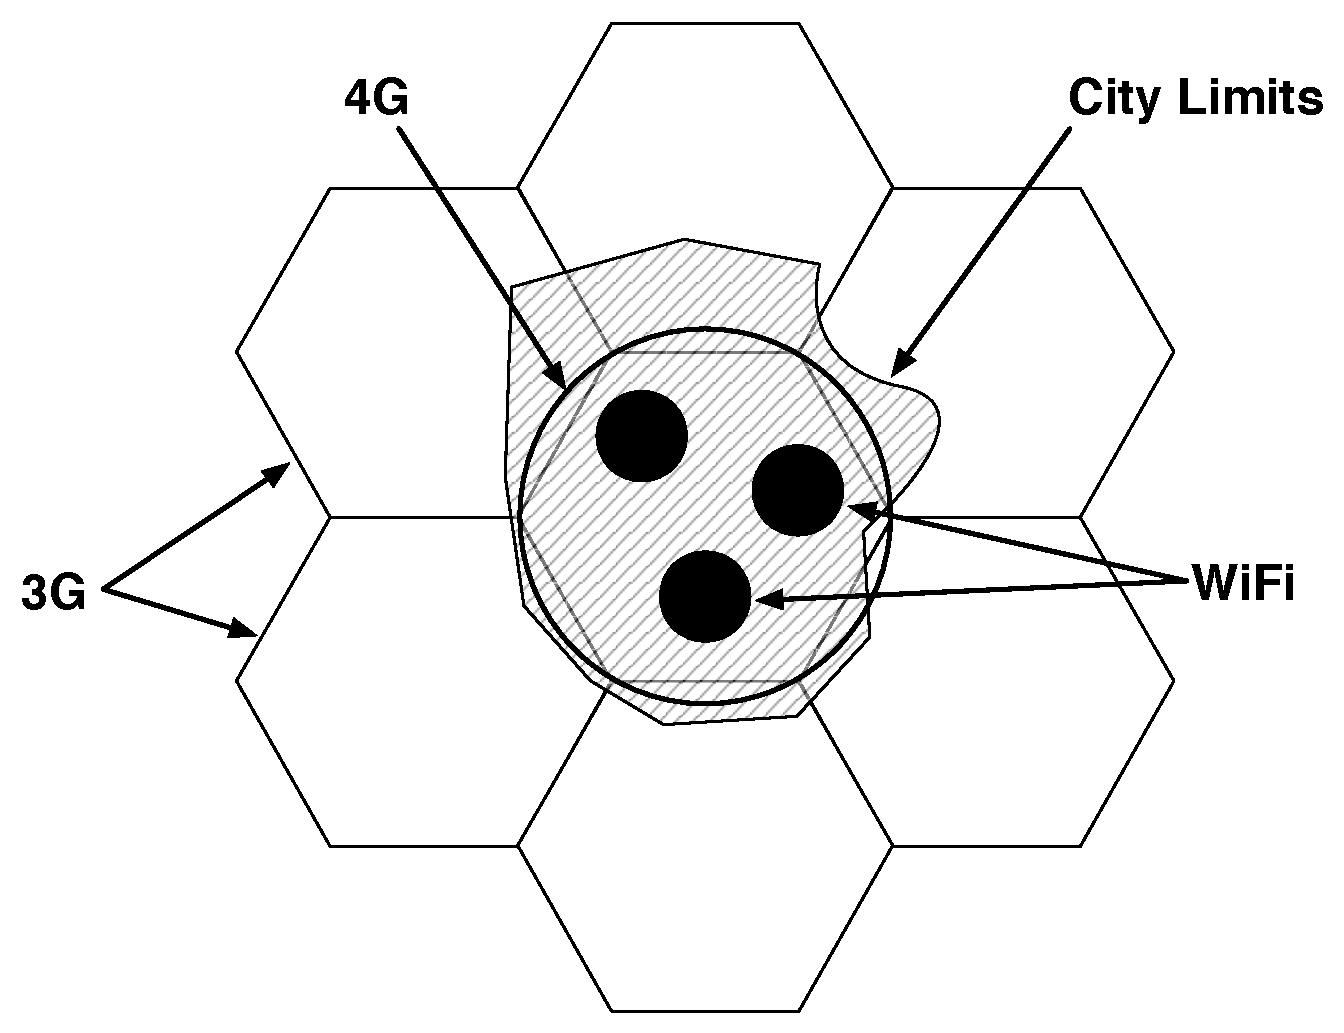
\includegraphics[width=4in]{Intelligent/Figures/wireless_city}
    \caption{Typical distribution of wireless access technologies in a modern-day city}
    \label{fig:wireless_city_intelligent}
\end{figure}

Figure~\ref{fig:wireless_city_intelligent} depicts a typical distribution of wireless access technologies in a modern-day city. In the example, WiFi hot spots are used as a localised very high-speed Internet access; 4G covers nearly the $\sfrac{3}{4}$ of the city area, and provides high-speed Internet access; and 3G delivers medium speed wireless access inside as well as outside the city. There is a high overlap of different wireless access technologies within the city. With the adoption of a heterogeneous wireless access network, this overlap could be utilised to its full potential by providing better network resources management, and high-speed and high quality Internet access for the users inside as well as outside the city limits.
% subsection heterogeneous_wireless_access_networks (end)

\subsection{Always Best Connected and Intelligent Network Selection} % (fold)
\label{sub:always_best_connected_and_intelligent_network_selection_intelligent}
As briefly mentioned in the previous section, \emph{Always Best Connected (ABC)} networking paradigm assumes that a wireless user is: (1) ``always'' connected to the Internet, and (2) uses the ``best'' access technology available \cite{ABC03}. ``Always'' should be interpreted as being able to utilise all wireless access technologies available at any time, while ``best'' implies that when a particular technology is being chosen, several factors such as user preferences, application requirements, network coverage, etc., are considered in order to make the most optimal selection possible (Figure~\ref{fig:abc_intelligent}). The mechanism responsible for implementing the ABC principles is referred to as \emph{intelligent network selection}.

\begin{figure}[ht]
    \centering
    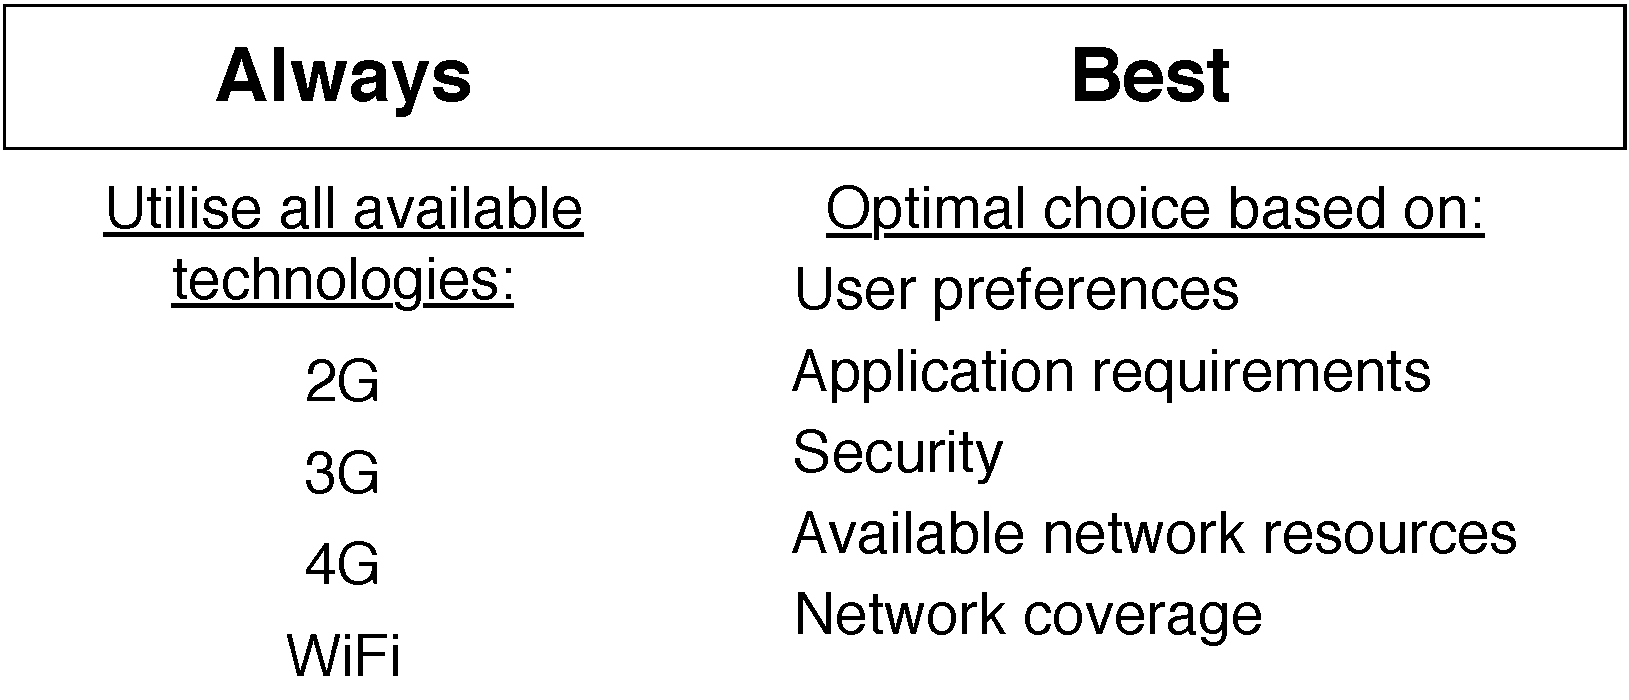
\includegraphics[width=4in]{Intelligent/Figures/abc}
    \caption{The essence of ABC networking paradigm}
    \label{fig:abc_intelligent}
\end{figure}

Furthermore, the paradigm emphasises seamless information delivery and extensive mobility support. In other words, the changes in the communications environment should affect the user as little as possible, even when they are ``on the move''. Therefore, should the user move from the coverage area of one access technology to another, the switch should be as non-disrupting for the user as possible; i.e., the session continuity should be maintained at all times, regardless of the access technology currently used. Thus, it is clear that intelligent network selection plays a vital role in the successful operation of the ABC solution.
% subsection always_best_connected_networking_paradigm (end)

\subsection{Tussle and Economic Aspects of Intelligent Network Selection} % (fold)
\label{sub:tussle_and_economic_aspects_of_intelligent_network_selection_intelligent}
While the integration of wireless access technologies into the heterogeneous wireless access network will lead to more efficient usage of network resources, the network operators will also be required to cooperate closely in order to manage such a complex system~\cite{HossainBeaubrun09,HossainTalebiFard09}. For example, new service agreements will need to be drafted to enable roaming access for users from and to the other network operators' networks.

Furthermore, since there are many different actors with opposing interests involved, there also exists the possibility of a `tussle'~\cite{Clark02}. For example, it is in the best interest of the users to obtain the highest quality of the service for the lowest price. Network operators, on the other hand, aim to maximize their profit by performing efficient load balancing. Furthermore, the situation may become even more complex should the service provision be decoupled from the network operators; that is, if the service provision is handled by a separate entity, service provider, while network operators are left with handling of the transport provision \cite{DMBushTussle09}. Therefore, the problem of intelligent network selection, which as pointed out in the previous section, was considered to be technologically difficult, can also be considered to be the problem of economics where wireless access, traded on a per connection basis, is an electronic good that is sold to the users.
% subsection tussle_and_economic_aspects_of_intelligent_network_selection (end)
% section the_problem_of_intelligent_network_seletion_intelligent (end)

\section{Intelligent Network Selection in the Literature} % (fold)
\label{sec:intelligent_network_selection_in_the_literature_intelligent}
Over the last decade, several papers have explored the problem of intelligent network selection in heterogeneous wireless access networks. Wang and Kuo provide an up-to-date survey of the mainstream approaches to the network selection problem covering: utility and game theory, fuzzy logic, multiple attribute decision making, combinatorial optimization, and Markov chains \cite{LushengKuo2013}. Liu \emph{et al.}, propose an algorithm for optimal network selection which mainly aims at optimizing energy consumption of the user equipment \cite{Liu2009}. Espi~\emph{et al.} present a machine learning approach to network selection; in particular, the authors utilize a Hopfield neural network to solve the underlying optimization problem \cite{Espi10}. Antoniou \emph{et al.}, and Charilas \emph{et al.}~model the problem as a noncooperative game between wireless access networks with the aim of obtaining the best possible trade-off between the efficiency and the available capacity of networks, while, at the same time, satisfying the requested quality by the subscribers \cite{Antoniou07, Charilas08}. Ormond \emph{et al.}~propose an algorithm for cost-oriented and performance-aware network selection that maximizes consumer surplus \cite{OrmondCS106, OrmondCS206}. Niyato \emph{et al.}~propose two algorithms based on evolutionary game theory for a network selection mechanism which performs intelligent load balancing so that network congestion and performance degradation can be avoided \cite{Niyato09}. Addtionally, the same authors model the user churning behavior in heterogeneous wireless access networks using evolutionary game theory \cite{NiyatoHossainConf2008}. Khan \emph{et al.}~model the problem as a procurement second-price sealed-bid auction where network operators bid for the right to service the subscriber's request \cite{Khan110, Khan210}. Zhu \emph{et al.}~build upon the work reported in~\cite{Niyato09}, and explore the dynamics of network selection, using Bayesian evolutionary game theory, in an environment where subscribers have only limited (incomplete) information about each others preferences \cite{ZhuNiyato2010}. Finally, Irvine \emph{et al.}~propose a market-based framework called the Digital Marketplace where network operators compete in a variant of a procurement first-price sealed-bid auction for the right to transport the subscriber's requested service over their infrastructure \cite{DMLeBodic00, DMIrvine01, DMIrvine02}.
% section intelligent_network_selection_in_the_literature_intelligent (end)

\section{Approaches Considering Economic Aspects} % (fold)
\label{sec:approaches_considering_economic_aspects_intelligent}

% section approaches_considering_economic_aspects_intelligent (end)

\section{Summary} % (fold)
\label{sec:summary_intelligent}

% section summary_intelligent (end)
% chapter intelligent (end)
